%----------------------------------------
% This is the skeleton for the AM-based track trigger
%----------------------------------------

\documentclass{cmspaper}
\usepackage{graphicx}
\usepackage{amssymb}
\usepackage{amsmath}
\usepackage{lineno}
\usepackage[table]{xcolor}
\linenumbers
\usepackage{url} 


\begin{document}

\begin{titlepage}
\internalnote{IN-2013/XXX}
%\cmsnote{2007/000}
\date{\today}
\title{Description of the CMS phase II track trigger system}
\begin{Authlist}
G.~Baulieu~\Aref{a}, C.~Combaret~\Aref{a}, R.~Dell~Orso~\Aref{b}, T.~Liu~\Aref{c}, L.~Martini~\Aref{b}, L.~Mirabito~\Aref{a}, F.~Palla~\Aref{b}, S.~Viret~\Aref{a}
\end{Authlist}

\Anotfoot{a}{Institut de Physique Nucl\'eaire, UCBL, CNRS-IN2P3, Lyon, France}
\Anotfoot{b}{INFN, Pisa, Italy}
\Anotfoot{c}{Fermilab, USA}

\begin{abstract}
The role of this note is to give an overview of the track-based triggering system at L1 for the CMS experiment. This study is entirely based on simulations results. The aim is to provide a detailed description of the system, along with estimation of the hardware system requirements. 
\end{abstract}
\end{titlepage}
\newpage
\tableofcontents
\newpage

%----------------------------------------
% Then you insert here the different parts of the report
%----------------------------------------

\section{Introduction}

\noindent Level-1 trigger (L1) is the first stage of CMS triggering system. This is a purely hardware stage during which LHC data rate is currently reduced from 20MHz to 100kHz within a latency of $6.4~\mu s$. Because of this very short latency, only the calorimeters and the muon subdetectors are part of L1 for the moment. The tracking detectors are used only at the second stage, knwon as the High-Level Trigger (HLT). 

\noindent Fig.~\ref{fig:L1Rates} illustrates how the lack of tracking at L1 might affect trigger efficiency. This figure shows, at LHC nominal luminosity, the rates of muons as a function of $p_T$. The line shows the generated muon rate, while black stars and red dots show muon rates after HLT and L1 respectively. The L1 muon rate, obtained using only the muon spectrometer, is much higher than the generated rate. It means that a lot of fake muons pass this trigger. These fakes are then cleaned at the HLT, as tracker info provides a much better sensitivity to muon identification than coarse muon info.
 
\begin{figure}[ht!]
\begin{minipage}[t]{7.5cm}
\centering
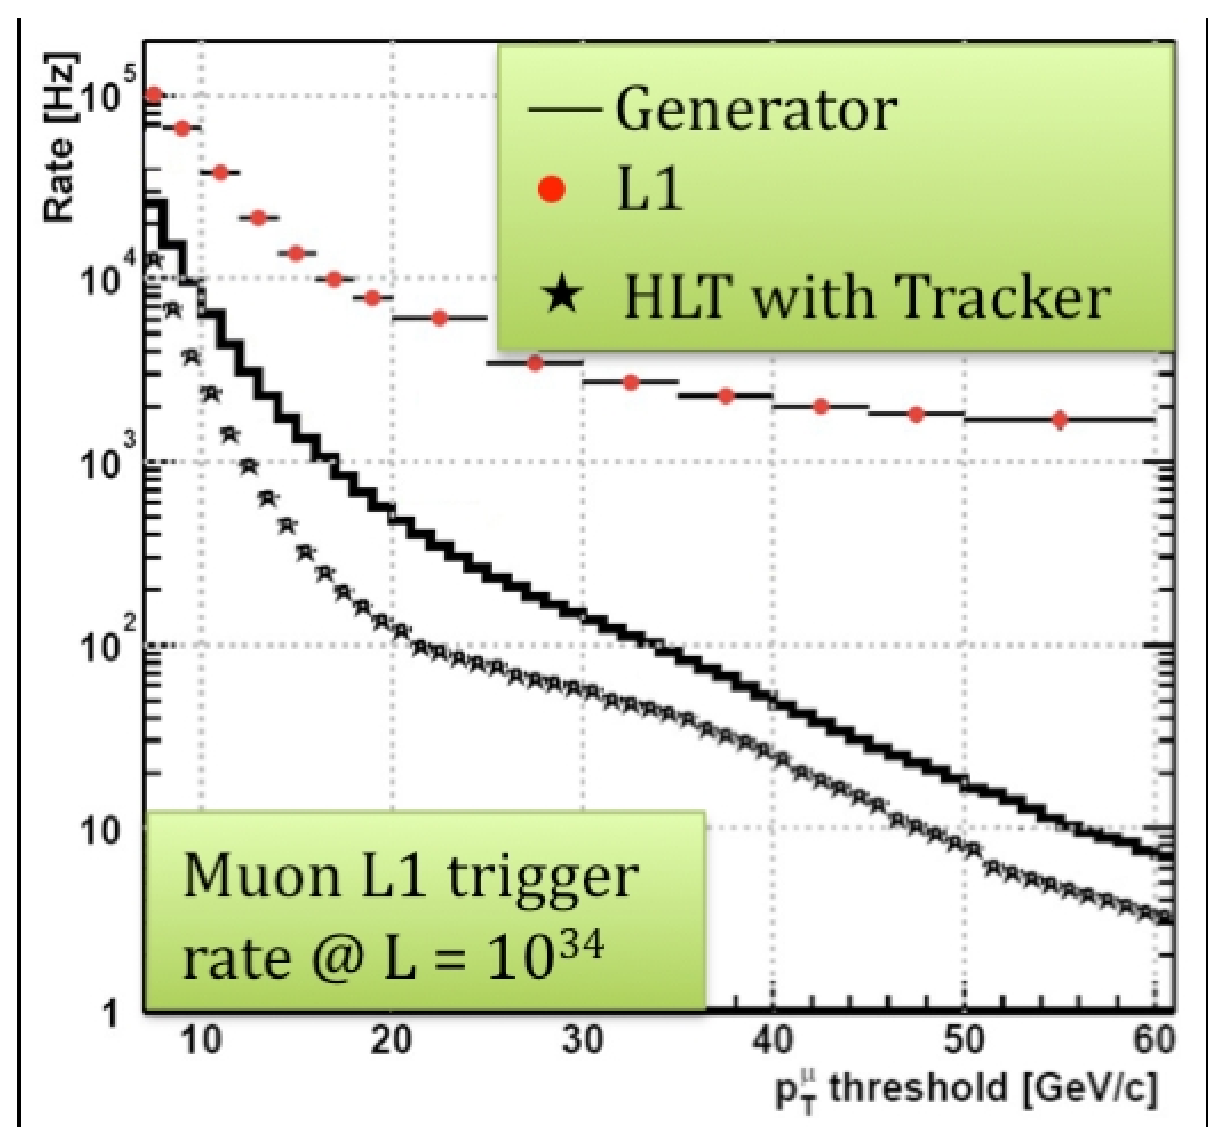
\includegraphics[width=0.99\textwidth]{Plots/CurrentTracker.eps}
\caption{Expected Level-1 single muon rate as a function of $p_{T}$ threshold for a luminosity of $10^{34}cm^{-2}s^{-1}$, in the present system.~\cite{bib:Abb-11}}
\label{fig:L1Rates}
\end{minipage}
\hfill
\begin{minipage}[t]{7.5cm}
\centering
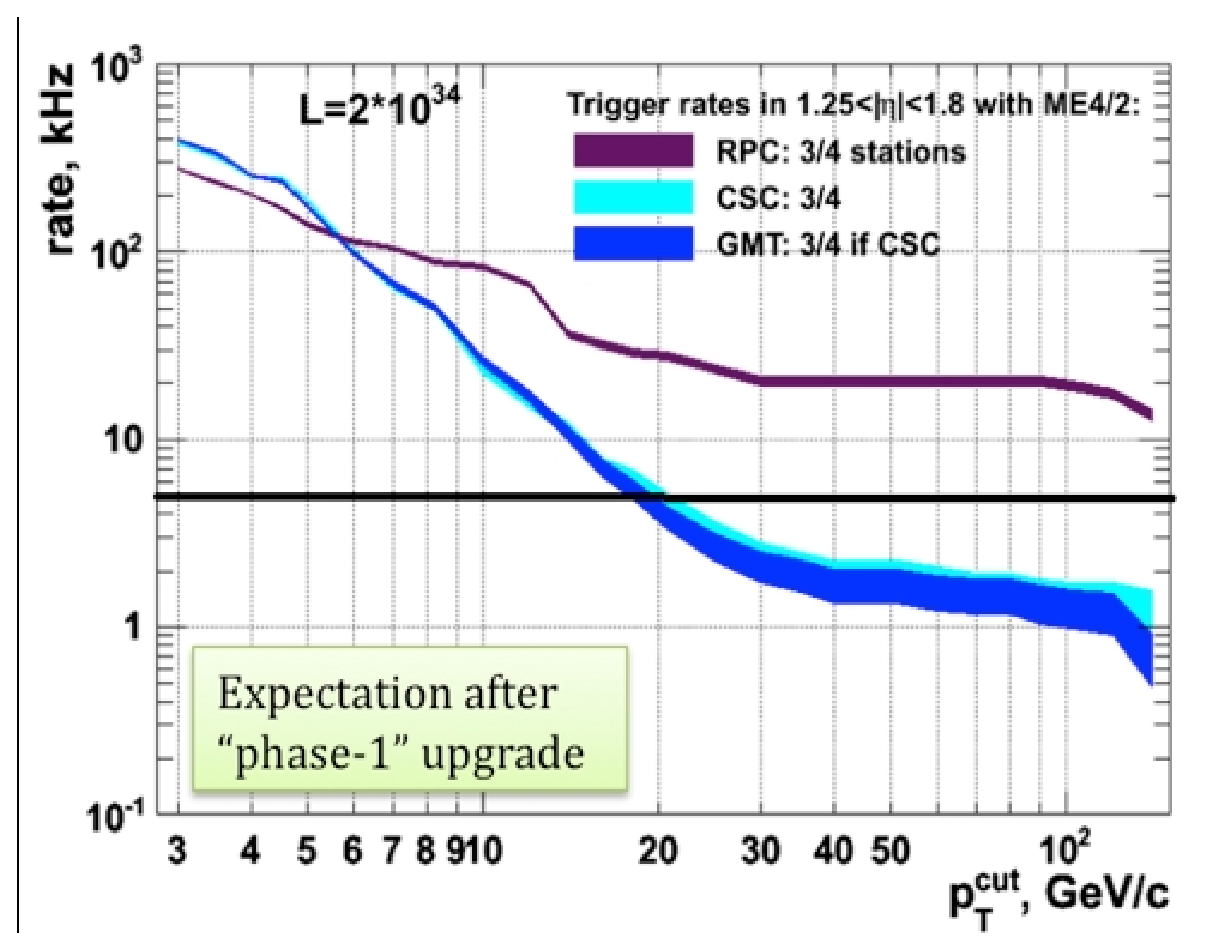
\includegraphics[width=0.99\textwidth]{Plots/21034_tracker.eps}
\caption{Expected threshold after phase 1 trigger upgrade, for a luminosity of $2\times 10^{34}cm^{-2}s^{-1}$.~\cite{bib:Abb-11}}
\label{fig:L1RatesPhase1}
\end{minipage}
\end{figure} 

\noindent One can also see on Fig.~\ref{fig:L1Rates} that fake proportion increases w.r.t. the $p_T$. This is due to the fact that L1 muon system uses coarse resolution information. Therefore high-$p_T$ tracks becomes compatible with straight lines at a certain point, and consequently the L1 muon rate reaches a plateau at high-$p_T$. At $10^{34}cm^{-2}s^{-1}$, this plateau lies at around $1~kHz$. Considering that overall L1 rate is $100~kHz$, the poor discrimination power at high-$p_T$ is not critical.

\noindent However, the plateau level is strongly depending on the instantaneous luminosity. Fig.~\ref{fig:L1RatesPhase1} shows its evolution, for the different muon subdetectors, at $2\times 10^{34}cm^{-2}s^{-1}$. For the RPC, the plateau lies at $20~kHz$, 20\% of the total L1 bandwidth. This is clearly not sustainable anymore. When going to HL-LHC luminosity, the other muons subdetectors also become problematic. In other words, muon indentification is not possible anymore. From there two solutions can be envisaged: increasing the L1 rate or including the tracking at L1. This note is dedicated to the second point.  

\noindent Our aim, in this document, is to procide a detailed description of such a system in the context of CMS. We tried to emulate the different stages of the hardware track fitting in order to estimate the feasibility/scaling of such a system with tracker geometry foreseen for CMS phase II upgrade. The simulation context, along with some estimation of the data rates that will be send to the trigger boards are presented in Section~{sec:FWork}. Pattern recognition is then described in Section~{sec:AM}. Finally, fitting stage is explained in Section~{sec:Fit}.

\clearpage

\section{System description}

\subsection{Overview}

\begin{figure}[ht!]
\centering
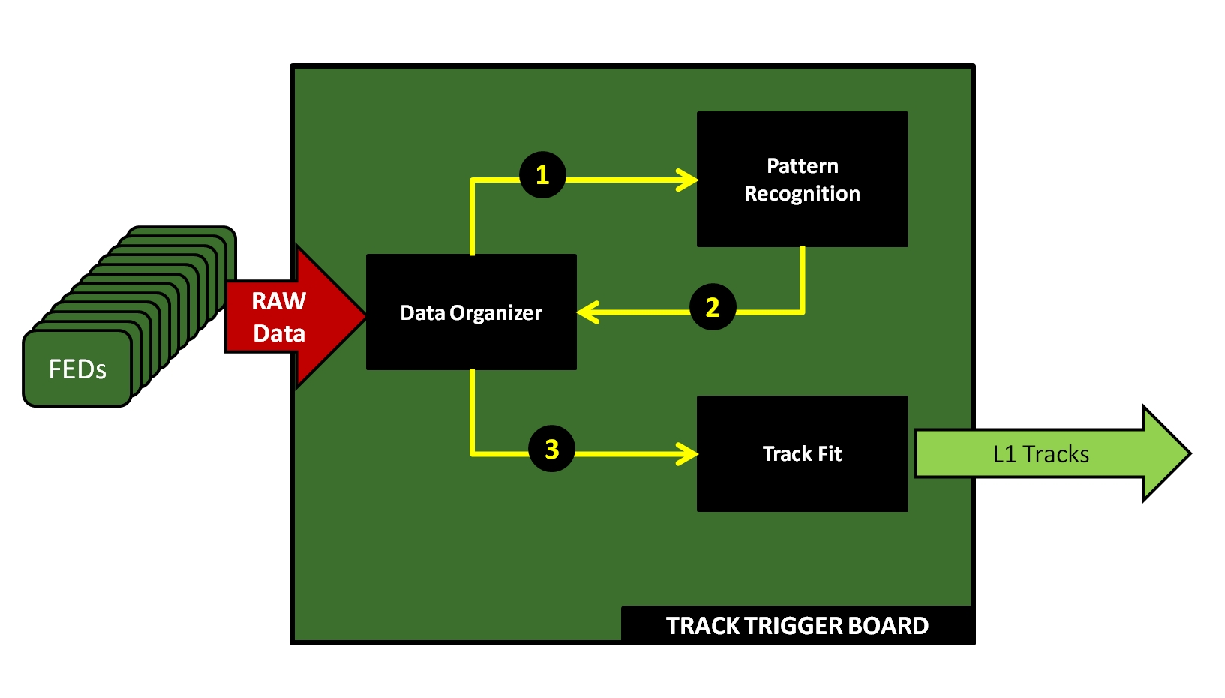
\includegraphics[width=0.5\columnwidth]{Plots/L1TTrigPrinciple.eps}
\caption{Hardware tracking principle}
\label{fig:L1TT_principle}
\end{figure}

\noindent Extracting track information is a two-stage process. First of all, you have to retrieve the hits belonging to the track: this is the pattern recognition. Then, you extract the track parameters (momentum, impact parameter,...) from the hits: this is the fit. Both steps are performed routinely in CMS, using very performant software algorithms. In order to pass to L1, tracking has to go hardware. Hardware-based tracking triggers were already developped in HEP experiments, in particular in the CDF experiment at Fermilab. Based on this system, the ATLAS experiment is planning to use a tracking trigger at the HLT after LHC long shutdown 2 in 2016. The working principle of these systems is sketched on Fig.~\ref{fig:L1TT_principle}. Tracker data is extracted by the FEDs and transmitted to the trigger board. Then, the data is handled by a data organization unit (DO), which extract the info necessary to the pattern recognition (PR), send it to the PR unit, and retrieve the matched patterns. The DO then sent the interesting hits to the track fit unit (TF), when the track parameters are estimated and sent to the L1 central trigger board.
\noindent In order to go at L1, one thus need the three following points: 

\begin{itemize}
\item A fast front-end readout system able to extract quickly all the data contained in the tracking detectors.
\item A system performing a fast pattern recognition.
\item A system performing a fast track fit.
\end{itemize}

\noindent Using associative memories in order to perform a fast pattern recognition (PR) at the trigger stage was first exposed in Ref.~\cite{bib:Del-89}. The principle is sketched in Fig.~\cite{fig:AM_principle}:
\begin{figure}[ht!]
\centering
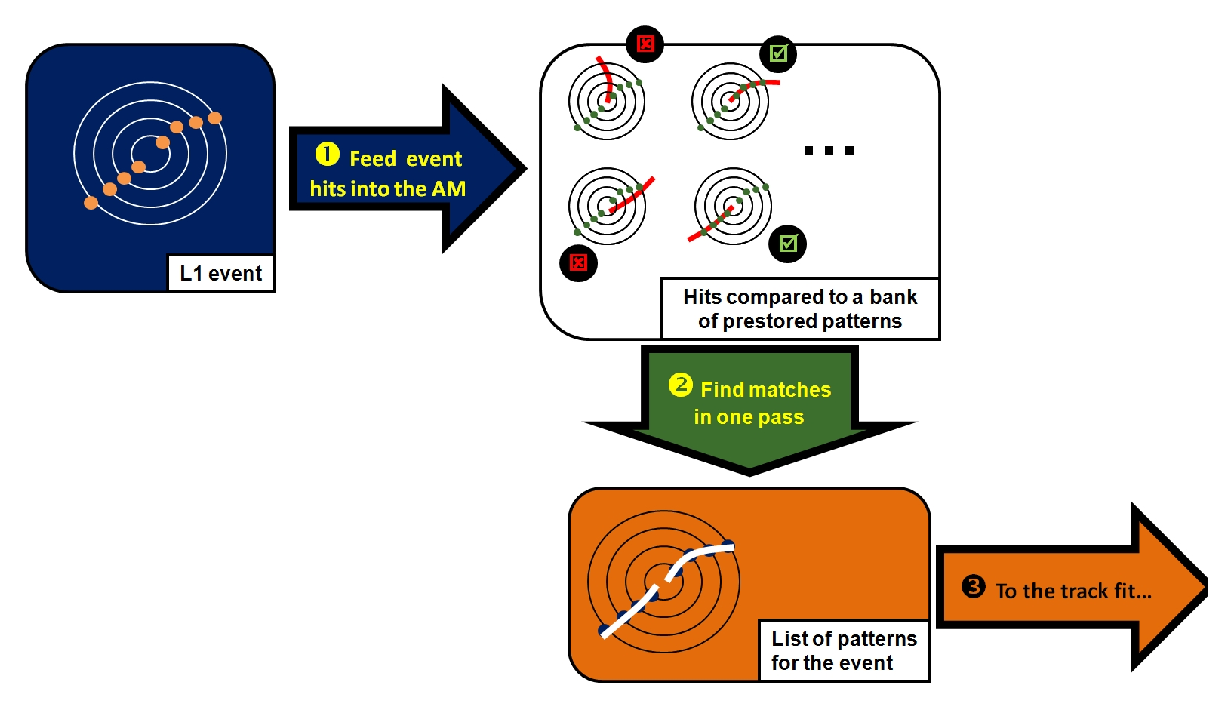
\includegraphics[width=0.7\columnwidth]{Plots/TriggerAM.eps}
\caption{Pattern recognition using associative memories.}
\label{fig:AM_principle}
\end{figure}

\noindent The idea is to compare the hits recorded in the tracking system to a bank of patterns stored in an associative memory chip. The patterns could be seen as low-granularity tracks, they are defined once for all using Monte-Carlo events, and they are ideally covering all the possible tracks occuring in the detector. In this part we will concentrate ourselves on the pattern bank definition. This is indeed the central point of the PR stage. The bank, which is defined using simulated events, has to fulfill few requirements. Before presenting them, it's important to define some parameters. 

\subsection{Data flow}

\subsection{Interface with Tracker FEDs and L1 Global Trigger}

\subsection{Simulation tools and needs}


\clearpage

\section{Performances}

\subsection{Tracking efficiency definition}

\subsection{Track trigger efficiency on single particles}

\subsection{Robustness against pile-up}

\subsection{Benchmark channel study}


\clearpage

\section{Hardware system description}
The associative memory system performs pattern recognition by comparing hits (stubs) with a reduced resolution with a large number
of prestored patterns almost in real time.

The system is composed of mainly three parts: a data formatter (DF), which prepares the data at the reduced granularity to be transferred 
to the Associative Memory chip (AMchip), where the comparison with the patterns is performed and a list of matched patterns
is returned back. The hits at full granularity are then retrieved from the DF for the final track fitting stage (TF).

\subsection{The AM chip}




\subsection{Trigger sectors}

\subsubsection{Definition}

\noindent The trigger definition is driven by two concurent constraints. As we will see later, the number of patterns will strongly depend on the sector size itself. It is therefore tempting to divide the detector into very small sectors, in order to work with small, easier to handle, banks. On the other hand, however, the minimal sector size will be geometrically constrained by the track trigger requirements. The system should indeed be able to detect tracks over a given $p_T$ threshold. The minimal sector should thus be able to entirely contain such tracks. For example, with a threshold of $2~GeV/c$, the minimal sector size is approximatively $18^{o}$.

\noindent This value sets the minimal overlap needed between two neghbouring sectors if one wants each track to be contained into at least one sector. In the following we divided the tracker into 8 sectors covering each $60^{o}$ in $\phi$, with therefore $20^{o}$ overlap between two consecutive sectors. The resulting division is shown on Fig.~\ref{fig:SEC_PHI}.

\begin{figure}[ht!]
\centering
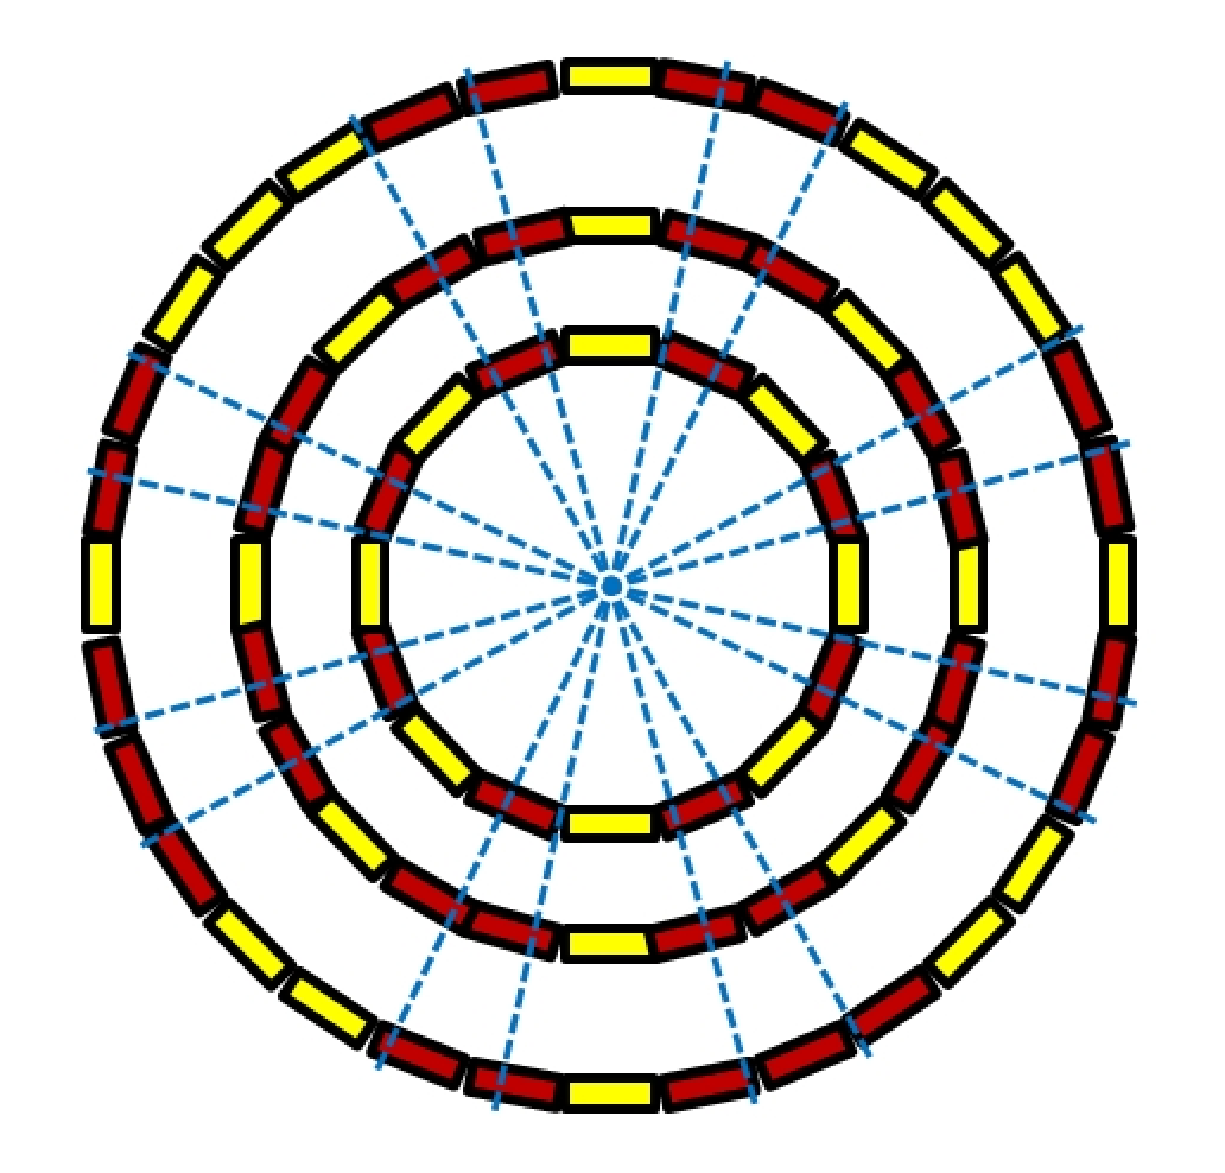
\includegraphics[width=0.5\textwidth]{Plots/AzimuthCut.eps}
\caption{\emph{Trigger sectors azimuthal division}}
\label{fig:SEC_PHI}
\end{figure} 

\noindent As one could see on Fig.~\ref{fig:SEC_PHI}, one has to take into account modules granularity into the sector definition. In the current simulation each sector is represented as a list of modules ID. These lists will be of particular importance for the definition of the FED to trigger boards mapping. Hopefully, once defined, they should be relatively stable along time. 

\begin{figure}[ht!]
\centering
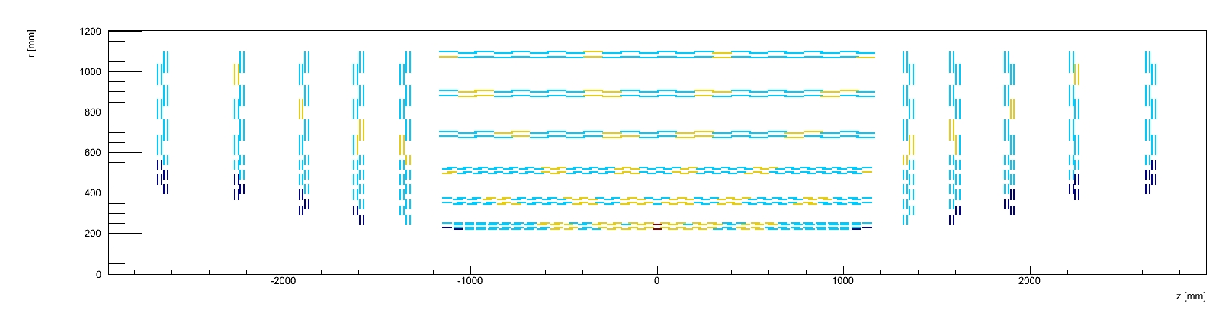
\includegraphics[width=0.9\textwidth]{Plots/EtaCut.eps}
\caption{\emph{Trigger sectors pseudo-rapidity division}}
\label{fig:SEC_ETA}
\end{figure} 

\noindent Using this configuration, we end up we 56 trigger sectors, 24 in the barrel, 16 in the endcaps, and 16 hybrids.

\subsubsection{Stub rates per sector in HL-LHC conditions}





\subsection{Patterns definition and generation}

\subsubsection{Pattern definition}

\noindent A pattern can be defined as a road in the sector. Each road may contain one or more tracks, as shown on the Fig.~\ref{fig:pattern}. 
\begin{figure}[ht!]
\centering
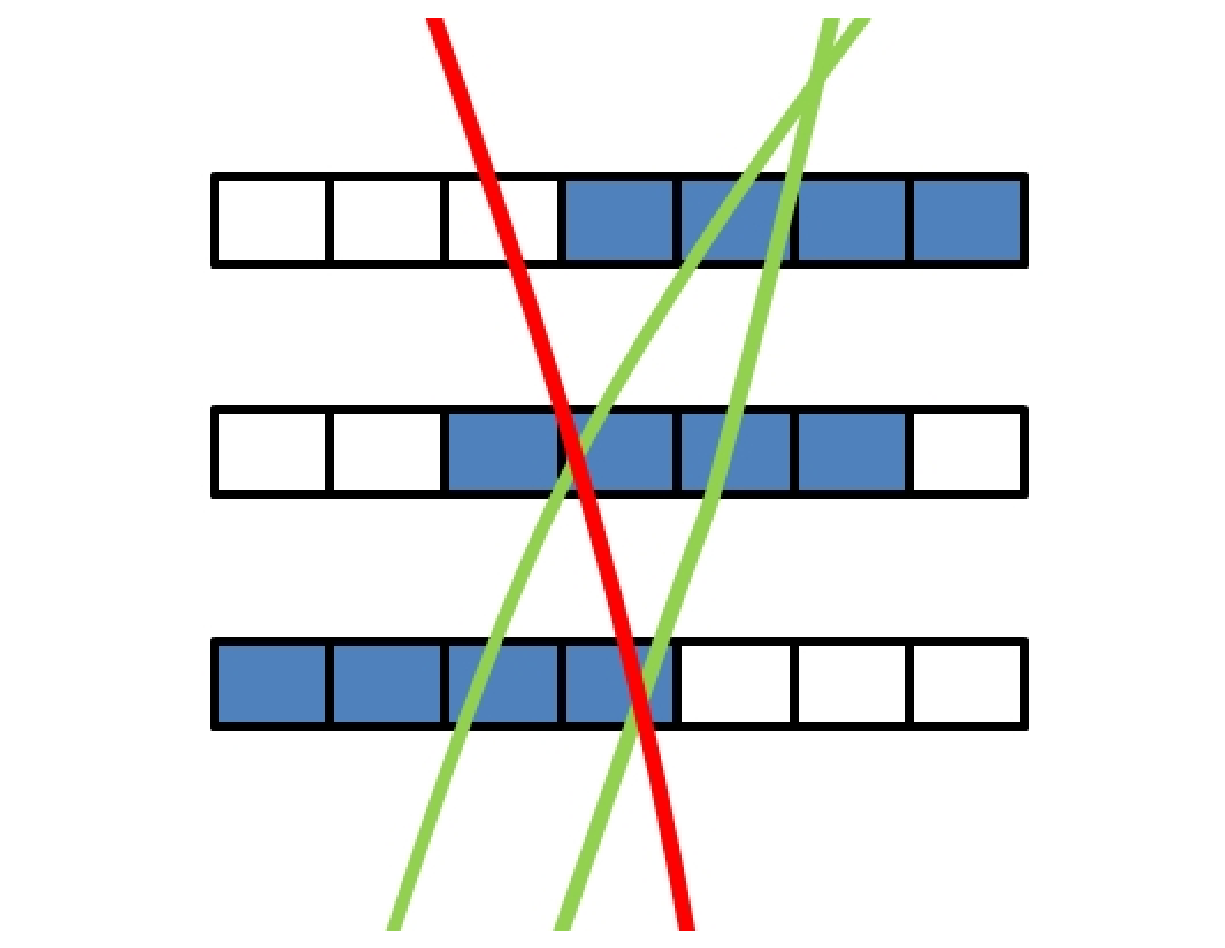
\includegraphics[width=0.3\columnwidth]{Plots/Pattern.eps}
\caption{A pattern in a three-layers detector. Green tracks will match the pattern, red tracks won't.}
\label{fig:pattern}
\end{figure}

\noindent On this picture one also get an idea of the pattern structure. Each pattern is made of one superstrip per layer. A superstrip is a group of strips/pixels, and is therefore heavily constrained by the detector itself. Once the superstrip definition has been set, its position information is coded in a N-bits word: the superstrip address. It is important to realize that the AM-based pattern recognition is using these addresses, and is therefore completely independent from the detector geometry.

\noindent As the addresses are transmitted to the AM independently for each layer, layer number doesn't have to be in the address word. In order to understand the address definition, Fig.~\ref{fig:sstrip_def} shows how a superstrip is defined in the barrel part of the tracker.  
\begin{figure}[ht!]
\centering
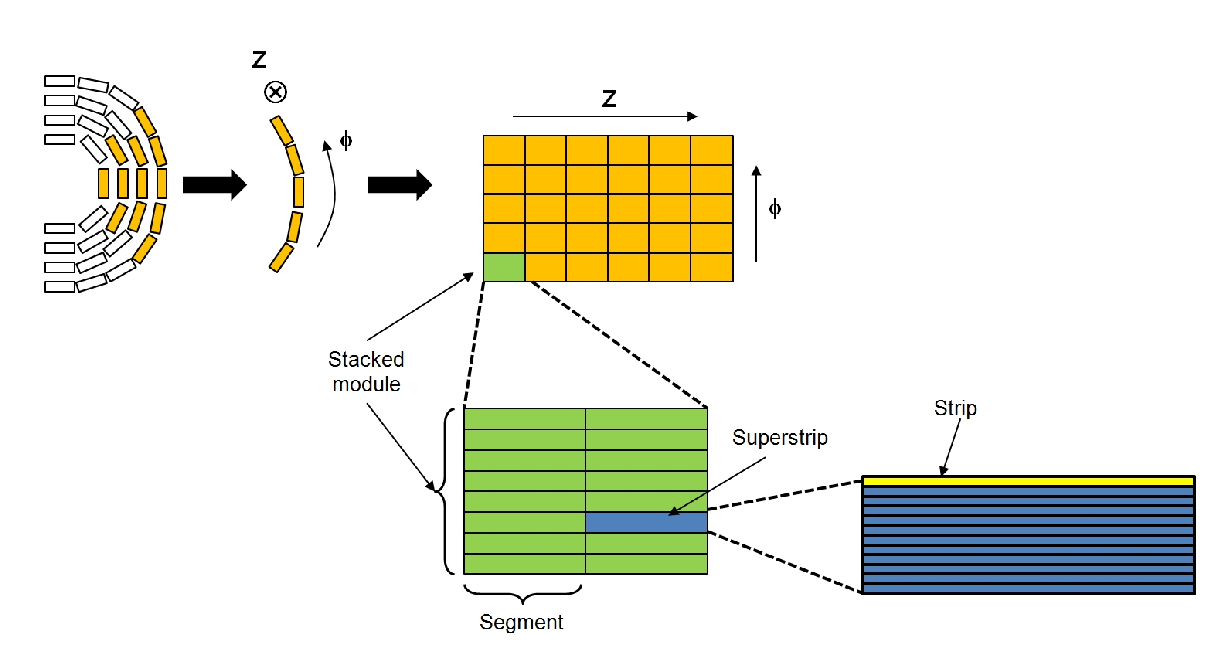
\includegraphics[width=0.7\columnwidth]{Plots/SStripDef.eps}
\caption{Geometric definition of a superstrip (barrel example).}
\label{fig:sstrip_def}
\end{figure}
\begin{figure}[ht!]
\centering
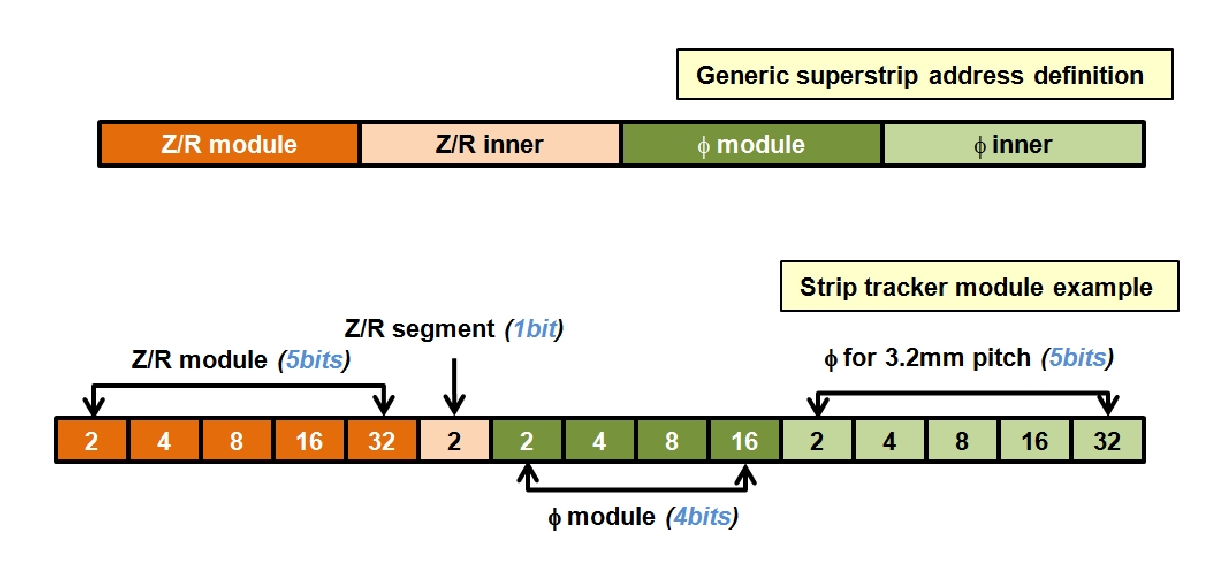
\includegraphics[width=0.7\columnwidth]{Plots/SSaddress.eps}
\caption{Address definition of a superstrip.}
\label{fig:SS_code}
\end{figure}

\noindent One has to be able to define a unique address to define the $z (resp. r)/\phi$ position of each superstrip in the barrel (resp. endcap) sector (r (resp. z) is given by the layer (resp. disk). The coding is sketched on Fig.~\ref{fig:SS_Code}. The number of bits necessary reflects the superstrip granularity and is constrained by the maximal word size acceptable by the AM chip (currently 16 bits). A first set of bits provides the module number along the corresponding coordinate: 5 bits for $Z$ (one could have up to 24 modules in Z in one sector) and 4 for $\phi$ (up to 11 modules per sector in the outermost layer). Then, for each coordinates, a second serie of bits provide the superstrip position within the module. Fig.~\ref{fig:sstrip_def} shows a tracker strip module (in green), divided into 2 segments in $Z$ and 1024 strip in $\phi$. Therefore in order to describe all the position, one would need only 1 bit for $Z$, and 10 bits for $\phi$. In practice, a certain number of strips are grouped to form the superstrip, in our case 32, thus leading to 5 in the address.   

\noindent For the endcap the coding is the same. z is just replaced by r (equivalence is made between disks and layers, ladders and rings). 

\subsubsection{Bank generation procedure}

\noindent The generation of the patterns bank is done using a Monte Carlo samples of particle gun $\mu^{\pm}$ produced within the following phase space:
\begin{itemize}
\item $0 < \eta_0 < 2.2$.
\item $1.95GeV/c < p_{T_0} < 100GeV/c$, generated randomly in $1/p_T$.
\item $-15cm < z_0 < 15cm$.
 \item $-1mm < d_0 < 1mm$.
\end{itemize}  

\noindent The direction of the transverse impulsion ($\phi_0$) is chosen such that the generated particles cover the sector we are interested in. The generation procedure is iterative and is using only tracks containing exactly one stub per layer/disk. At iteration $n$, a set of $N$ such tracks is collected. Then one computes the PR efficiency for those tracks using the pattern bank obtained at the end of iteration $n-1$. If the efficiency is larger than a given threshold (called the coverage), the procedure stops. Otherwise, the new patterns formed with those tracks are added to the bank and iteration $n+1$ is done. 

\noindent At the beginning of the first iteration, the bank being empty, every particle will lead to a new pattern insertion. Then, as the bank is being populated, the efficiency growth will become slower.

\subsubsection{Bank efficiency definition}

\noindent Let's denote $N$ the number of tracks you want to reconstruct in a given event, ie the tracks which are within the L1 track trigger requirements. Then, we denote $N^{matched}$ the number of tracks which are contained into at least one pattern. The PR efficiency $\epsilon$ can thus be defined as: 
\begin{equation}
\epsilon = \frac{N^{matched}}{N}
\end{equation} 

\noindent Then, we note $N_{pattern}$ the total number of patterns activated in the event and $N^{matching}_{pattern}$ the number of patterns containing one of the tracks we are looking for. From there one could define the fake rate $\rho$:
\begin{equation}
\rho = 1 - \frac{N^{matching}_{pattern}}{N_{pattern}}
\end{equation} 

\noindent Another important figure is the redundancy $r$. It corresponds to the average number of patterns activated by a good track. 

\noindent Last but not least, one should keep in mind that the PR goal is to provide low-sized hit sets for the track fitting (TF) stage in order to reduce the combinatorics, and consequently the TF time budget. The proportion of good hits per pattern, noted $\epsilon_{hits}$ is therefore a very important parameter:
\begin{equation}
\epsilon_{hits} = \frac{1}{N_{pattern}}\sum_{N_{pattern}}\frac{N_{hits}^{good}}{N_{hits}}
\end{equation} 

\noindent The ideal pattern bank is the one for which:  
\begin{enumerate}
\item $\epsilon = 1$.
\item $\rho = 0$.
\item $r = 1$.
\item $\epsilon_{hits} = 1$. 
\end{enumerate}  

\noindent This ideal bank exists, this is the one for which each possible track in the detector corresponds to one pattern. However, the size of such bank is clearly prohibitive. On the other side, one could imagine the simplest bank with 1 single pattern defined by the whole detector. Such a bank will have $\epsilon=1$, $\rho = 0$ and $r = 1$, but $\epsilon_{hits}$ will be close to 0. Such a solution would be highly inefficient, as TF would be impossible to process. Therefore the optimal solution lies in between, and one realizes that a parameter will be very important: the size of the patterns. The patterns will have to be sufficiently small in order to get a reasonable $\epsilon_{hits}$, but also sufficiently large in order get a reasonable pattern bank size. 

\subsubsection{Bank size with 6 layers}

\subsection{Track fitter module}

\subsection{Timing considerations}

\subsection{Overall board/crate layout}


\clearpage

\section{Integration, development, and cost estimate}

\subsection{Project planning}

\subsection{System tests and feasibility setups}

\clearpage

\section{Conclusion}

\clearpage



%----------------------------------------
% Bibliography
%----------------------------------------

\newpage
\thispagestyle{empty}

\begin{thebibliography}{99}

%\bibitem{bib:Abb-11} D.~Abbaneo {\it for the CMS collaboration} - {\it "Upgrade of the CMS Tracker with tracking trigger"} - CMS CR -2011/284 (2011)

%\bibitem{bib:Del-89} M. Dell Orso, L. Ristori - {\it "VLSI Structure For Track Finding"} - Nucl.Instr. and Meth. A278 (1989), 436

%\bibitem{bib:XML_wiki}\url{https://twiki.cern.ch/twiki/bin/view/CMSPublic/SWGuideGeomDevelopersGuide}

%\bibitem{bib:XML_oscar}\url{https://twiki.cern.ch/twiki/bin/view/CMSPublic/SWGuideOscarProducer}

%\bibitem{bib:G4SHits_cfi}\url{http://cmssw.cvs.cern.ch/cgi-bin/cmssw.cgi/CMSSW/SimG4Core/Application/python/g4SimHits_cfi.py?view=markup}

%\bibitem{bib:ANN-08} A. Annovi {\it et al.} - {\it "A new Variable Resolution Associative Memory for High Energy Physics"} - ATL-UPGRADE-PROC-2011-004 (2011)

%\bibitem{bib:Kar-91} V.~Karimaki - {\it "Effective circle fitting for particle trajectories"} - Nucl.Instr. and Meth. A305 (1991), 187

\end{thebibliography}
%----------------------------------------
% Annexes
%----------------------------------------

%\appendix


\end{document}
